\section{Klassenattribute und Klassenoperationen}
\label{sec:Kap-8.3}

Bisher haben wir Attribute betrachtet, die zwar durch die Klasse definiert werden, für die aber jede Instanz der Klasse ihre eigenen Wertebelegungen haben kann. Das Klassenkonzept der Objektorientierung sieht neben diesen Attributen, die man auch Instanzattribute nennen kann, noch eine andere Art von Attributen vor, die sogenannten \textit{Klassenattribute}. Ein Klassenattribut ist ein Attribut, das in der Klasse verortet ist und dessen Wert von allen Instanzen der Klasse geteilt wird. Im Unter\-schied zu Instanzattributen besitzt also nicht jede Instanz eine eigene Wertebelegung für dieses Attribut, sondern es existiert nur ein gemeinsamer Wert. Wird dieser Wert verändert, haben alle Instanzen der Klasse eine neue Wertebelegung in dem entsprechenden Attribut. Klassenattribute verwendet man für die Abbildung von Eigenschaften, die relevant für die inhaltliche Modellierung einer konkreten \mbox{Klasse} sind, sich aber nicht den einzelnen Instanzen der Klasse zuordnen lassen. Ein Klassen\-attribut existiert auch dann, wenn (noch) keine Instanz der Klasse erzeugt wurde. 

\vspace{\baselineskip} %%% für Druck
\vspace{2mm} %%% für Druck

\begin{figure}[h!]
	\centering
	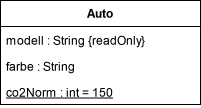
\includegraphics[scale=1.0]{Bilder/Kapitel-8/klasse_auto_mit_klassenattribut.pdf}
	\caption{Klassenattribut}
	\label{fig:klasse_auto_mit_klassenattribut}
\end{figure}

\vspace{2mm} %%% für Druck

Ein Klassenattribut in unserem Autobeispiel-Kontext könnte \sttpUMLText{co2Norm} sein, wenn wir idealisiert annehmen, dass für alle Automodelle eine einheitliche $\text{CO}_2$-Abgasnorm gilt (Abb.~\ref{fig:klasse_auto_mit_klassenattribut}). Klassenattribute werden in der UML-Darstellung der Klasse unter\-strichen. In der Darstellung der Instanzen wird ein Klassenattribut identisch zu den Instanzattributen dargestellt, also nicht unterstrichen. Häufig wird ein Klassen\-attribut aber aus Redundanzgründen (da es für jede Instanz denselben Wert hat) gar nicht in der Darstellung der Instanzen aufgeführt. Neben den Klassen\-attributen gibt es auch \textit{Klassenoperationen}. Klassenoperationen werden auf der Klasse und nicht auf einer konkreten Instanz aufgerufen. Sie werden verwendet, um auf die Klassenattribute zuzugreifen. Wie die Klassenattribute werden Klassenoperationen in der UML-Darstellung unterstrichen.

\vspace{2mm} %%% für Druck

Eine 
\marginline{Konstruktoren, Destruktoren}
besondere Form von Operationen sind die Operationen zum Erzeugen und Löschen von Instanzen, die sogenannten Konstruktoren und Destruktoren. In manchen objektorientierten Programmiersprachen entspricht ihre Syntax der Syntax von Klassenoperationen. In Java haben Konstruktoren eine spezielle Syntax, die sich von derjenigen der Klassenoperationen unterscheidet. Zudem kennt Java keine Destruktoren, sondern stattdessen das Konzept des Garbage Collectors, nicht mehr verwendete Instanzen werden automatisch gefunden und zerstört. Konstruktoren und Destruktoren werden aus Übersichtlichkeitsgründen üblicherweise nicht im UML-Klassendiagramm aufgeführt.